\section{The Duffing oscillator}

\subsection{Analytical Ansatz}
As we have seen, Josephson junctions act as nonlinear inductors, hence adding nonlinearity, or anharmonicity, to an electrical circuit.
When the circuit is driven with low enough input power, the nonlinearity can be neglected.
In this case, the circuit can be described well by a driven harmonic oscillator,
\begin{align}
\ddot{x} + \delta \dot{x} + \alpha x = \gamma \cos(\omega t),
\end{align}
with the time-dependent displacement  $x=x(t)$, stiffness $\alpha$, damping $\delta$, drive amplitude $\gamma$ and drive frequency $\omega$.
All variables are assumed to be positive and real.
However, for most cases it is important to account for the anharmonicity.
The generalized mathematical model which describes such a circuit is the Duffing equation with the following equation of motion (EOM)\cite{hamelGeorgDuffingIngenieur1921}:
\begin{align}
\ddot{x} + \delta \dot{x} + \alpha x + \beta x^3 = \gamma \cos(\omega t),
\end{align}
with the anharmonicity $\beta$.

In fact, there exists an algebraic equation describing the amplitude response\cite{jordanNonlinearOrdinaryDifferential2007,rajasekarHarmonicNonlinearResonances2016}:
\begin{align}
\left[ \left( \omega^2-\alpha-\frac{3}{4}\beta x^2 \right)^2 + \left( \delta\omega \right)^2 \right] x^2 = \gamma^2
\label{eq:Duffing-analytical}
\end{align}
We plot the solutions to a set of parameters ($\alpha=\gamma=1,\delta=0.1$) in Fig.\ref{fig:duffing}.

\begin{figure}
	\centering
	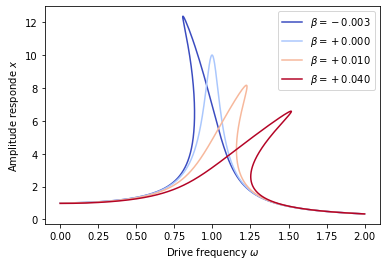
\includegraphics[width=0.7\linewidth]{chapter-theory/figs-general/duffing}
	\caption{Frequency response of Duffing oscillators for various nonlinearities and $\alpha=\gamma=1,\delta=0.1$, calculated from Eq.\ref{eq:Duffing-analytical}}
	\label{fig:duffing}
\end{figure}

\subsection{Intuitive Ansatz}
We can also take a more intuitive Ansatz to the above problem from which we can already gain qualitative information.
Let us assume the Duffing equation describes a mass on a (nonlinear) spring driven by a periodic external force.
Compared to the linear case with $F_r=kx$, the new restoring force is now given by 
\begin{align}
F_r = k^\prime x = (\alpha +\beta x^2)x.
\end{align}
For $\beta>0$, the spring is stiffened, for $\beta<0$ the spring is softened.
Quantitatively, the sign of $\beta$ does not have any effect on the behaviour of the circuit for frequency shifts small compared to the resonance frequency of the circuit.
Following first order perturbation theory, let us assume 
\begin{align}
x=x_0 \cos(\omega t)% + x_1\cos(3\omega t) + \dots
\end{align}
to be the solution of the unperturbed EOM.
If we insert this into the equation for the restoring force, we need to first calculate
\begin{align}
x^2(t) = x_0^2\cos^2(\omega t) = x_0^2\frac{1}{2}(1+2\cos(2\omega t))
\end{align}
Compared to $\cos(\omega t)$, the time average of $\cos(2\omega t)$ is zero.
Thus, the restoring force is given by
\begin{align}
F_r=k^\prime x \approx \left(k+\frac{\beta x_0^2}{2}\right)x
\end{align}
and the corresponding resonance frequency
\begin{align}
\omega \approx \omega_0 + \diff{\omega}{k}\Delta k \approx \omega_0 + \frac{\omega_0}{2}\frac{\Delta k}{k} = \omega_0 \left(1+\frac{\beta x_0^2}{4k}\right).
\end{align}
We see that the resonance frequency of the unperturbed system experiences a shift proportional to $\beta$ and the square of the position, $x_0^2$.

\section{Anharmonicities in cQED}

In the field of circuit quantum electrondynamics (cQED), the above mentioned nonlinearities or anharmonicities can be analytically calculated for any circuit.

The general way of calculation is to convert the circuit to be evaluated into a one where the source of anharmonicity (namely the Josephson junction) is in parallel to the rest of the circuit.
The anharmonicity is then given by
\begin{align}
A=-\frac{2e^2}{L_j\omega_0^2\left[\text{Im} Y^\prime(\omega_0)\right]^2},
\end{align}
with the circuit admittance $Y=1/Z$, resonance frequency $\omega_0$ and $Y^\prime(\omega_0)=\diff{Y}{\omega}(\omega_0)$.

\subsection{Transmon qubit}

\begin{align}
Z=\sqrt{\frac{nL_j}{C}}
\end{align}
The voltage drop across the $i$th JJ is
\begin{align}
\phi_\text{zpf}^{(i)} = \frac{1}{n}\times\phi_\text{zpf}^\text{node}
\end{align}
with $\phi_\text{zpf}^\text{node}$ the zero point fluctuations across the entire circuit.
For our circuit Hamiltonian it then follows 
\begin{align}
\mathcal{H}&= \frac{E_J}{2} \sum_{i} \left( \frac{\phi_\text{zpf}^{(i)}}{\Phi_0} \right)^4 \left(\hat{a}^\dagger+\hat{a}\right)^4
\end{align}
and only looking at the terms with $\hat{a}^\dagger \hat{a}^\dagger \hat{a} \hat{a}$, the anharmonicity is given by
\begin{align}
\frac{A}{2} &=\frac{E_J}{\Phi_0}\times n \times \left(\sqrt{\frac{\hbar}{2} \sqrt{\frac{nL_j}{C}}}\times \frac{1}{n}\right)^4  \\
&= E_c \times \frac{1}{n^3}
\end{align}
with the charging energy $E_c=e^2/(2C)$.

\subsection{DC bias cavity + a few JJs}\label{sec:distributed}

As long as the impedance of the Josephson junctions, $Z_J=i\omega L\ll Z_{TL}$, we can model our CPW shorted by Josephson junctions as a series LC-resonator, where the junction array is added in series to the resonator inductance.
The total characteristic impedance is thus described via
\begin{align}
Z=\sqrt{\frac{L+nL_j}{C}}
\end{align}
Since this circuit is essentially a voltage divider, the voltage drop across the $i$th JJ is
\begin{align}
\phi_\text{zpf}^{(i)} = \phi_\text{zpf}^\text{node}\times\frac{Z^{(i)}}{Z}=\phi_\text{zpf}^\text{node}\times\frac{L_j}{L+n L_j}
\end{align}
with $\phi_\text{zpf}^\text{node}$ the zero point fluctuations across the entire circuit.
For our circuit Hamiltonian it then follows 
\begin{align}
\mathcal{H}&= \frac{E_J}{2} \sum_{i} \left( \frac{\phi_\text{zpf}^{(i)}}{\Phi_0} \right)^4 \left(\hat{a}^\dagger+\hat{a}\right)^4
\end{align}
and only looking at the terms with $\hat{a}^\dagger \hat{a}^\dagger \hat{a} \hat{a}$, the anharmonicity is given by
\begin{align}
\frac{A}{2} &=\frac{E_J}{\Phi_0}\times n \times \left(\sqrt{\frac{\hbar}{2} \sqrt{\frac{L+nL_j}{C}}}\times \frac{L_J}{L+nL_j}\right)^4  \\
&= \frac{E_J}{\Phi_0}\times n \times \left(\sqrt{\frac{\hbar}{2} \sqrt{\frac{L_j}{C}}}\times \left(\frac{L_J}{L+nL_j}\right)^{3/4}\right)^4  \\
A &= E_c \times n \left(\frac{L_J}{L+nL_j}\right)^{3}
\end{align}
with the charging energy $E_c=e^2/(2C)$.

\subsection{Inductively side-coupled Josephson array}\label{sec:lumped}

For the case of the lumped device, where the Josephson array is parallel to the resonator inductance, the corresponding total inductance is
\begin{align}
L^*=\frac{L \times nL_j}{L+nL_j}
\end{align}
and the zero point fluctuations of each individual junction
\begin{align}
\phi_\text{zpf}^{(i)}=\frac{1}{n}\phi_\text{zpf}^\text{node}
\end{align}

The contribution to the anharmonicity is then
\begin{align}
A&=E_J \sum_{i} \left( \frac{\phi_\text{zpf}^{(i)}}{\Phi_0} \right)^4 \\
&=E_J \times n \times \frac{1}{n^4} \left( \frac{\phi_\text{zpf}^\text{node}}{\Phi_0} \right)^4 \\
&= E_j\times\frac{1}{n^3} \left( \sqrt{\frac{\hbar}{2} \sqrt{\frac{L_j}{C}} } \right)^4 \times \frac{1}{\Phi_0^4} \times \left( \sqrt{\sqrt{\frac{nL}{L+nL_j}}} \right)^4 \\
A&= E_c \times \frac{1}{n^2}\frac{L}{L+nL_j}
\end{align}

%\bibliography{dissertation}